% \part*{Inleiding}

% % % % % % % % % % % % % % % % % % % % % % % % % % % % % % % % %
% % % % % % % % % % % % % % % % % % % % % % % % % % % % % % % % %
% % % % % % % % % % % % % % % % % % % % % % % % % % % % % % % % %
% % % % % % % % % % % % % % % % % % % % % % % % % % % % % % % % %
% % % % % % % % % % % % % % % % % % % % % % % % % % % % % % % % %
% % % % % % % % % % % % % % % % % % % % % % % % % % % % % % % % %
% % % % % % % % % % % % % % % % % % % % % % % % % % % % % % % % %
% % % % % % % % % % % % % % % % % % % % % % % % % % % % % % % % %
% % % % % % % % % % % % % % % % % % % % % % % % % % % % % % % % %
% % % % % % % % % % % % % % % % % % % % % % % % % % % % % % % % %
% % % % % % % % % % % % % % % % % % % % % % % % % % % % % % % % %
% % % % % % % % % % % % % % % % % % % % % % % % % % % % % %

\begin{figure}[h!]
    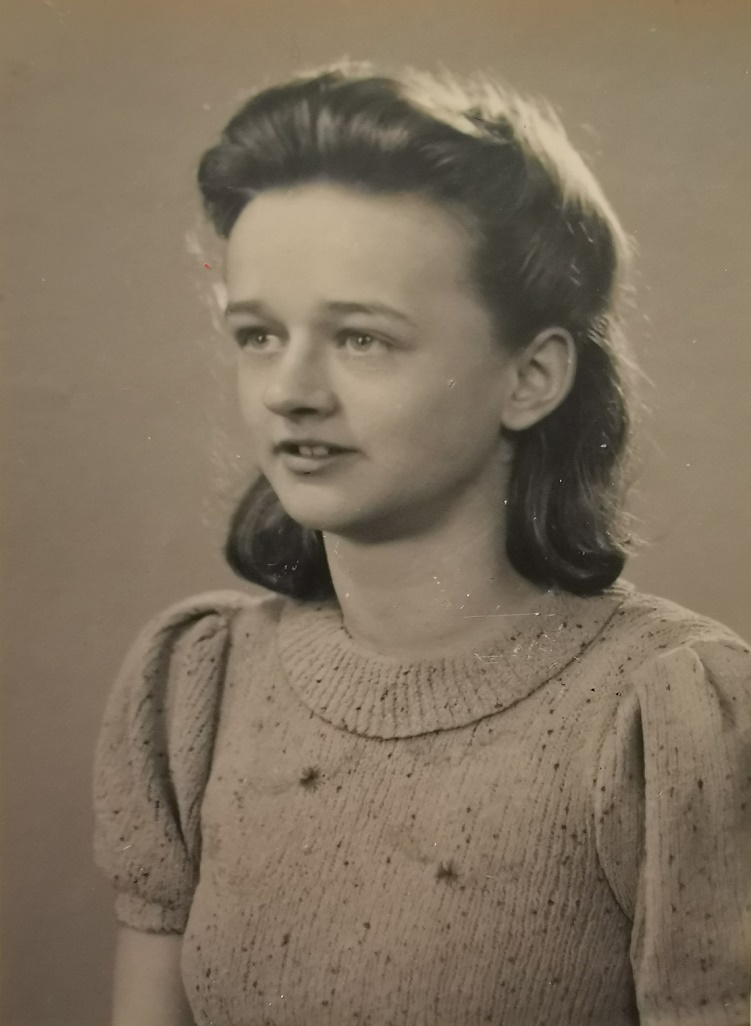
\includegraphics[width=\textwidth]{image1.jpeg}
    \caption{Tine de Booij}
\end{figure}

\chapter*{Inleiding} 

In dit boek vertel ik, Tine de Booij, over mijn leven.
Het boek is opgebouwd uit interviews door mijn dochters Jacqueline en Yvonne en door mijn kleinkinderen Lisa, Anneflore en Dorus. Timon heeft de lay-out gemaakt. En ik heb de eindcontrole gedaan.

Voor ons allemaal bijzonder om zo samen in het verleden te graven.
Af en toe leek het wel een officieel interview.
Het leidde ook tot mooie gesprekken over dingen waar we het nooit over hadden gehad.
Veel leesplezier!
